% !TeX program = lualatex
\documentclass[tikz,border=2pt]{standalone}

\usepackage{pgfplots,amsmath}
\pgfplotsset{compat=1.18}
\usetikzlibrary{shapes.geometric}
\usepgfplotslibrary{fillbetween}
\usepackage[colorlinks=true,linkcolor=blue,urlcolor=blue]{hyperref}

\begin{document}

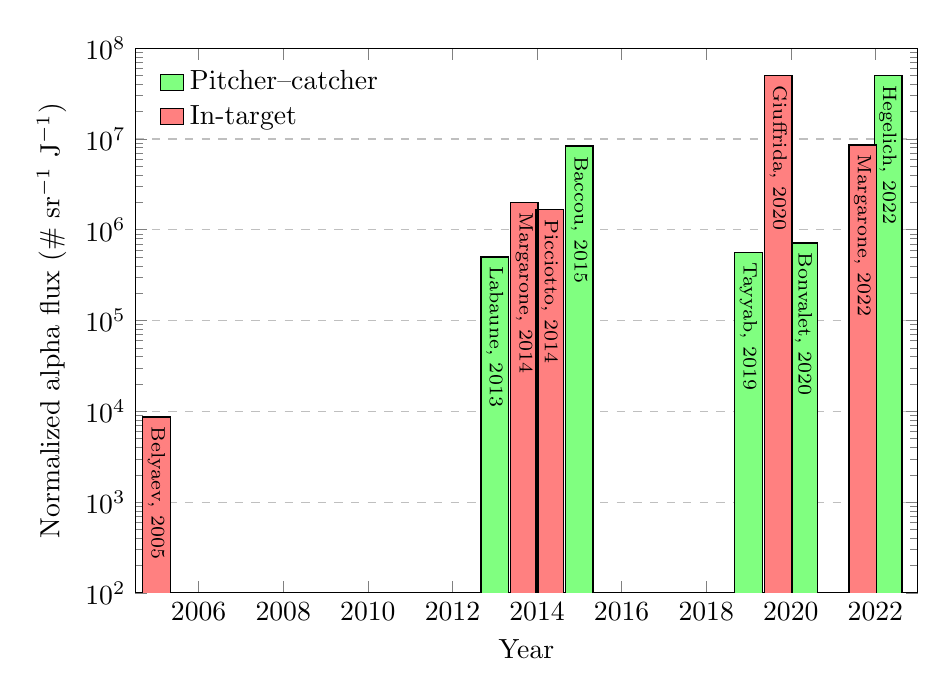
\begin{tikzpicture}
\pgfplotsset{compat=1.18}
\begin{axis}[
  width=0.95\linewidth,
  height=8.5cm,
  ymode=log,
  ymin=1e2, ymax=1e8,
  xmin=2004.5, xmax=2023,
  xtick={2006,2008,2010,2012,2014,2016,2018,2020,2022,2024},
  xticklabels={2006,2008,2010,2012,2014,2016,2018,2020,2022,2024},
  xlabel={Year},
  ylabel={Normalized alpha flux (\# sr$^{-1}$ J$^{-1}$)},
  ymajorgrids=true,
  grid style={dashed,gray!50},
  bar width=10pt,
  legend style={at={(0.02,0.98)}, anchor=north west, draw=none, fill=none, cells={anchor=west}},
  legend image code/.code={
    \draw[#1,fill=#1,draw=black,line width=0.4pt] (0cm,-0.1cm) rectangle (0.3cm,0.1cm);
  },
  nodes near coords,
  nodes near coords style={font=\scriptsize, rotate=-90, color=black, anchor=west},
  every node near coord/.append style={/pgf/number format/precision=3}
]

% ---------------------------------
% Pitcher-catcher (green bars)
% Labels provided via "explicit symbolic" meta
% ---------------------------------
\addplot+[
  ybar,
  fill=green!50,
  draw=black,
  line width=0.5pt,
  mark=none,
  point meta=explicit symbolic
] coordinates {
  (2022.3, 5.0e7)   [Hegelich, 2022]
  (2020.3, 7.14e5)  [Bonvalet, 2020]
  (2019, 5.6e5)   [Tayyab, 2019]
  (2015, 8.33e6)  [Baccou, 2015]
  (2013, 5.0e5)   [Labaune, 2013]
};
\addlegendentry{Pitcher--catcher}

% ---------------------------------
% In-target (red bars)
% ---------------------------------
\addplot+[
  ybar,
  fill=red!50,
  draw=black,
  line width=0.5pt,
  mark=none,
  point meta=explicit symbolic
] coordinates {
  (2021.7, 8.57e6)  [Margarone, 2022]
  (2019.7, 5.0e7)   [Giuffrida, 2020]
  (2013.7, 2.0e6)   [Margarone, 2014]
  (2014.3, 1.67e6)[Picciotto, 2014]
  (2005, 8.67e3)  [Belyaev, 2005]
};
\addlegendentry{In-target}

\end{axis}
\end{tikzpicture}

\end{document}